\documentclass[12pt]{article}
\usepackage[magyar]{babel}
\usepackage{t1enc}
\usepackage{graphicx}
\usepackage{enumitem}
\usepackage{spverbatim}
\usepackage[headheight=20pt]{geometry}
\usepackage{fancyhdr}
\usepackage[colorlinks,linkcolor=black,%
urlcolor=blue,citecolor=orange,linktoc=all]{hyperref}

\pagestyle{fancy}
\fancyhf{}
\fancypagestyle{plain}{%
\fancyhf{}%
\fancyhf[CH]{Beadandó}%
\fancyhf[LH]{Adatbázisrendszerek I}%
\fancyhf[RH]{Sindely Richárd - P1UV07}%
\fancyhf[CF]{Miskolci Egyetem}%
\fancyhf[RF]{\thepage}%
}
\renewcommand{\footrulewidth}{0.4pt}
\fancyhf[CH]{Beadandó}
\fancyhf[LH]{Adatbázisrendszerek I}
\fancyhf[RH]{Sindely Richárd - P1UV07}
\fancyhf[CF]{Miskolci Egyetem}
\fancyhf[RF]{\thepage}

\author{Sindely Richárd-P1UV07}
\title{Adatbázisrendszerek I. beadandó}
\date{2023}

\begin{document}
\maketitle
\newpage
\tableofcontents
\newpage
\section{Bevezetés}
\label{bev}
Az adatbázisomhoz a volánbusz rendszere adott inspirációt, amelyben van egy \textbf{Utas} egyed, amely a következő tulajdonságokkal rendelkezik:
\begin{itemize}
\item uid (PK - Elsődleges kulcs)
\item név (Az utas neve)
\item szülév (Utas születési éve)
\item személyi ig. szám (Az utas szemlyi ig. száma)
\item telefonszám (Utas telefonszáma,többértékű)
\item kor (Leszármaztatott érték)
\item jegy/bérlet típusa
\end{itemize}
A következő egyed a \textbf{Busz} ami egy adott buszról tartalmaz információkat.
\begin{itemize}
\item bid (PK - Elsődleges kulcs)
\item rendszám (Busz rendszáma)
\item típusszám (Busz típus/gyártási száma)
\item márka (Busz gyártója)
\end{itemize}
Van még egy \textbf{Söfőr} egyed ami a céghez tartozó buszsöfőröket tartja számon, melynek a tulajdonságai a következők:
\begin{itemize}
\item sid (PK - Elsődleges kulcs)
\item név (Söfőr neve)
\item kezdés éve (Az év amikor a söfőr elkezdett dolgozni a cégnél)
\item ledolgozott évek száma (Leszármaztatott érték)
\end{itemize}
Következő egyed az a \textbf{Járatszám} ami a következő tulajdonságokkal rendelkezik:
\begin{itemize}
\item jid (PK - Elsődleges kulcs)
\item szam (Járatnak a száma)
\end{itemize}
Az \textbf{Utas} és a \textbf{Járatszám} egyedek között van egy kapcsolat ami tartalmaz egy tulajdonságot ami a:
\begin{itemize}
\item ülés (Ülés száma ahova az utas ül)
\end{itemize}
A \textbf{Megállók} egyed a következő tulajdonságokkal bír:
\begin{itemize}
\item mid (PK - Elsődleges kulcs)
\item koordináta (Megálló helyzetének koordinátája)
\item név (Megálló neve)
\end{itemize}
A \textbf{Járatszám} és a \textbf{Megállók} egyedek között van egy kapcsolat ami kettő tulajdonságot is tartalmaz:
\begin{itemize}
\item tervezett indulás
\item tervezett érkezés
\end{itemize}
Végül a \textbf{Települések} egyed tartalmazza a települések tulajdonságait amelyek a következők:
\begin{itemize}
\item tid (PK - Elsődleges kulcs)
\item irányítószám (Települések irányítószáma)
\item név (Települések neve)
\end{itemize}
\newpage
\section{ER diagram}
Előzőleg bemutatott egyedek, tulajdonságok ER diagrammja:\\
\\
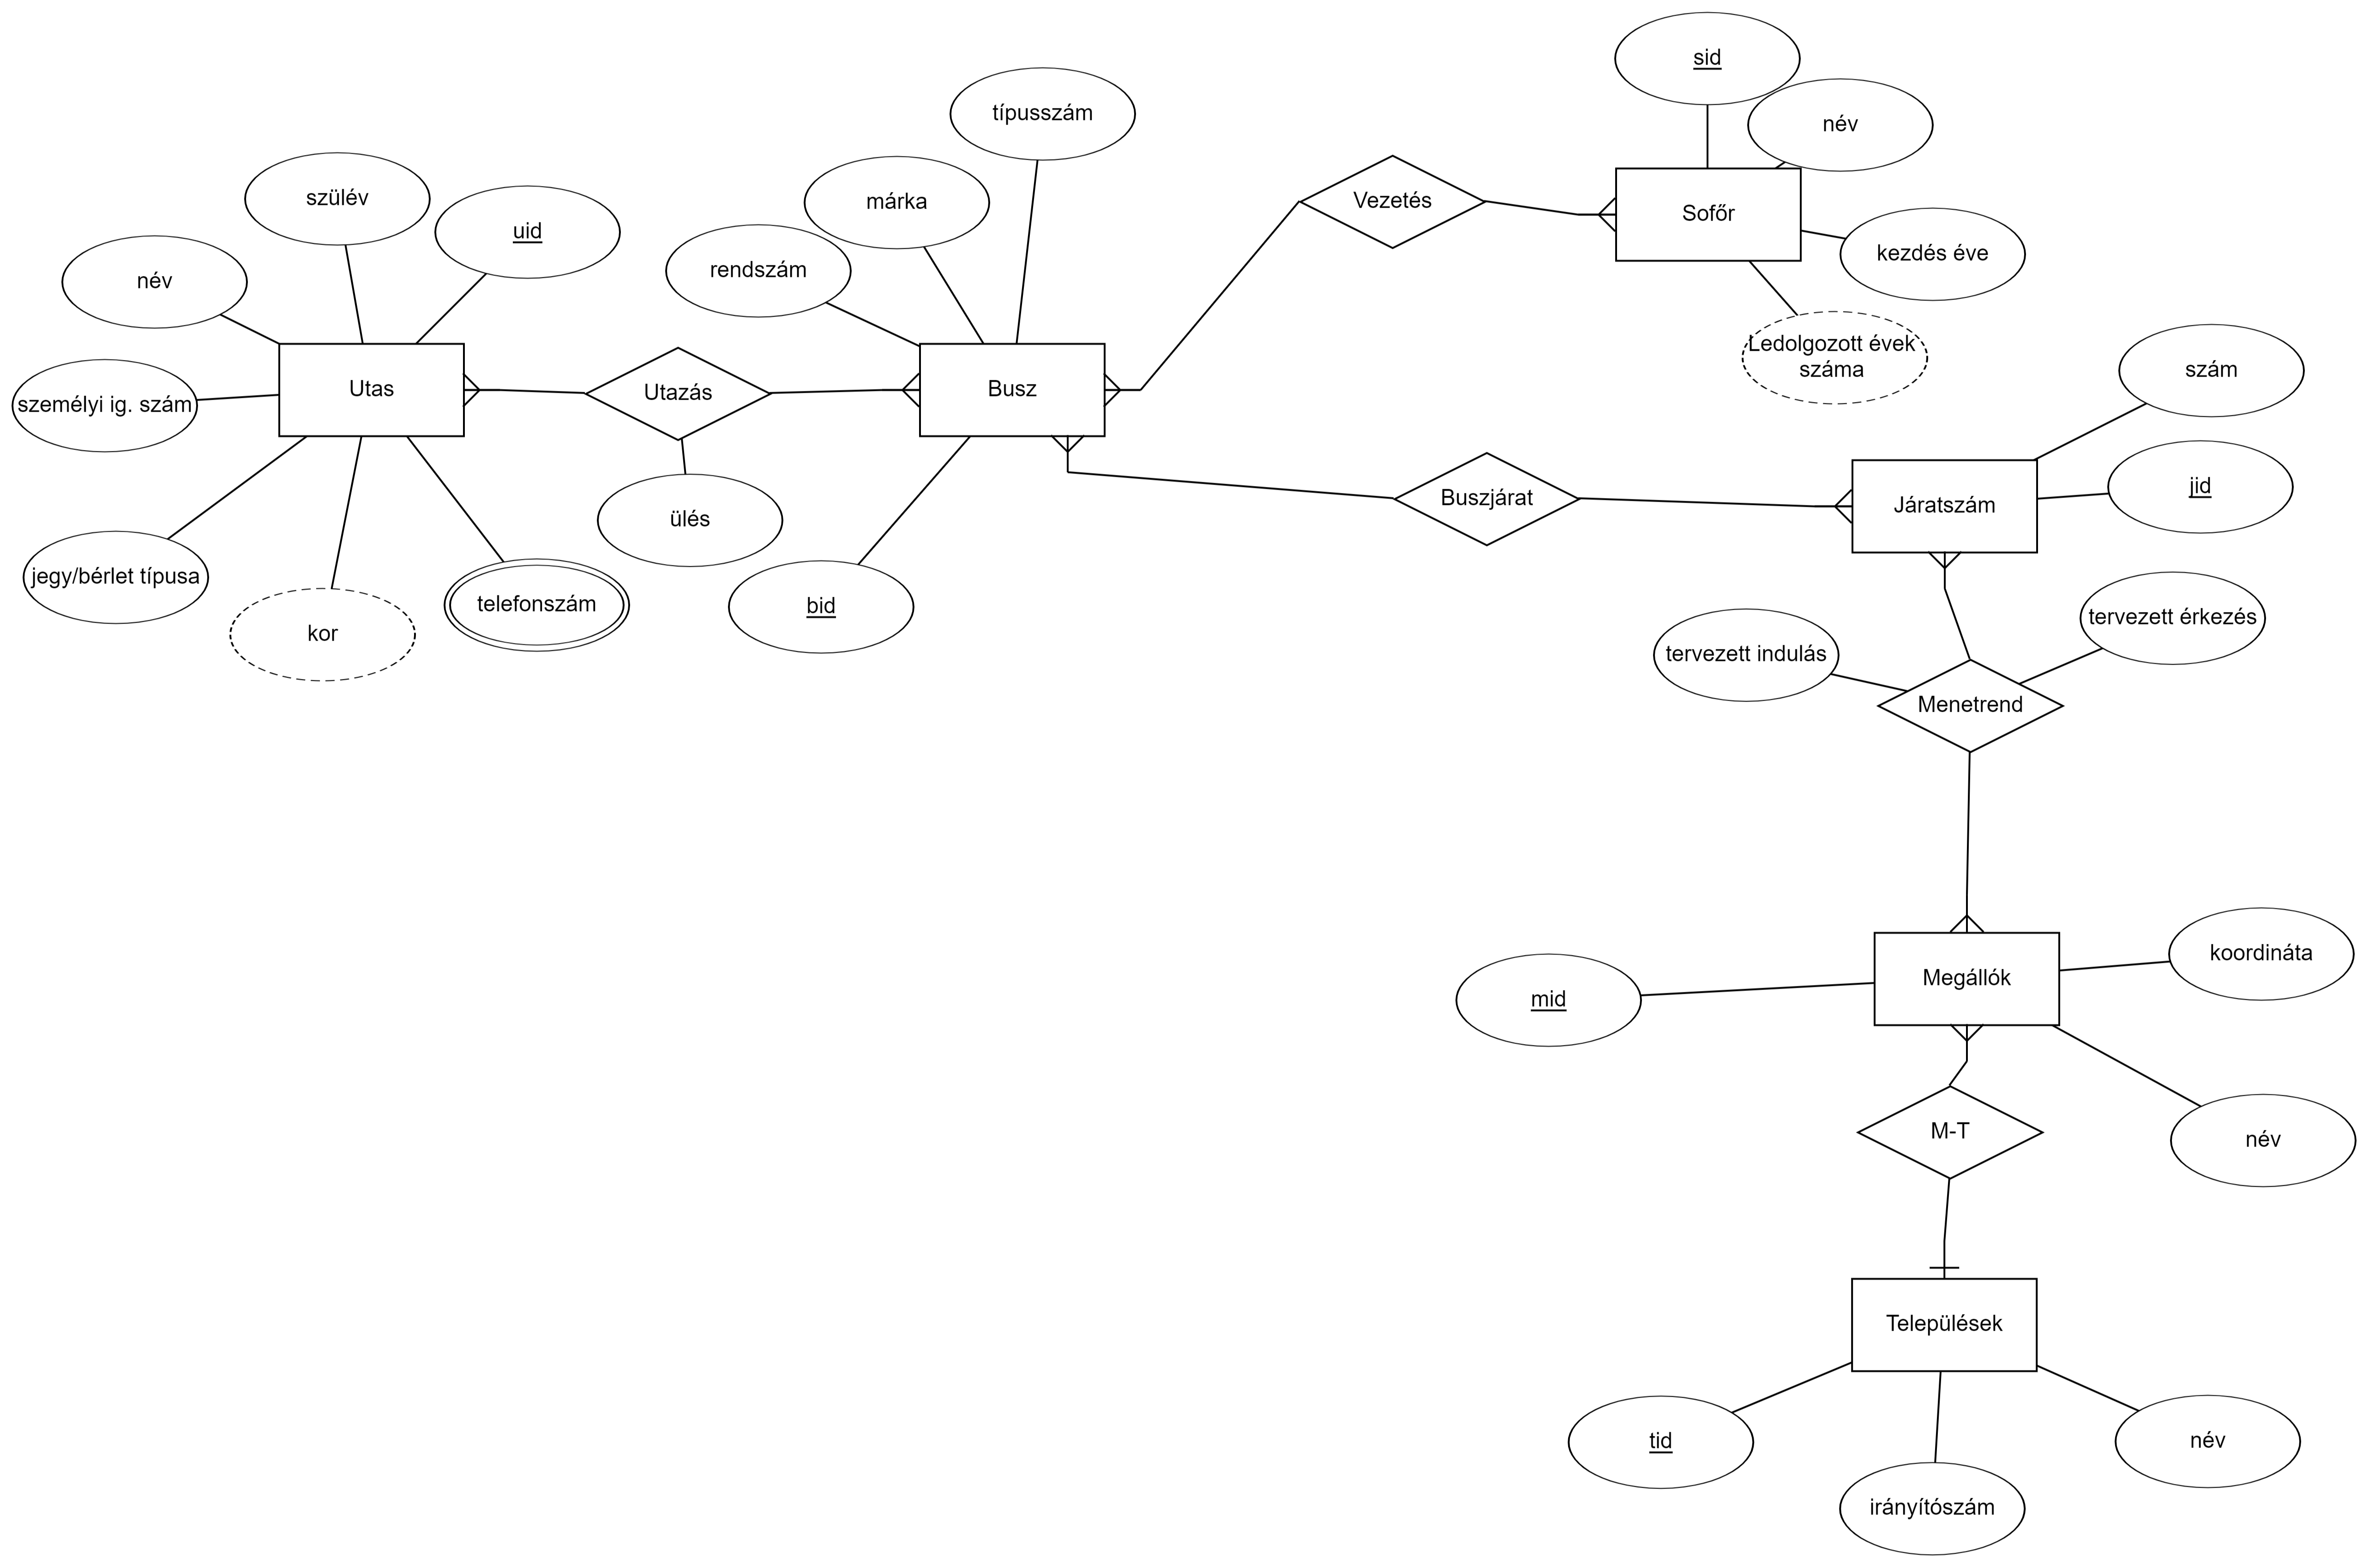
\includegraphics[height=15cm,width=15cm]{D:/Uni/Tex/Adatbázis beadandó/er.png}
\newpage
\section{RS diagram}
Bevezetésben bemutatott egyedek, tulajdonságok RS diagramja:\\
\\
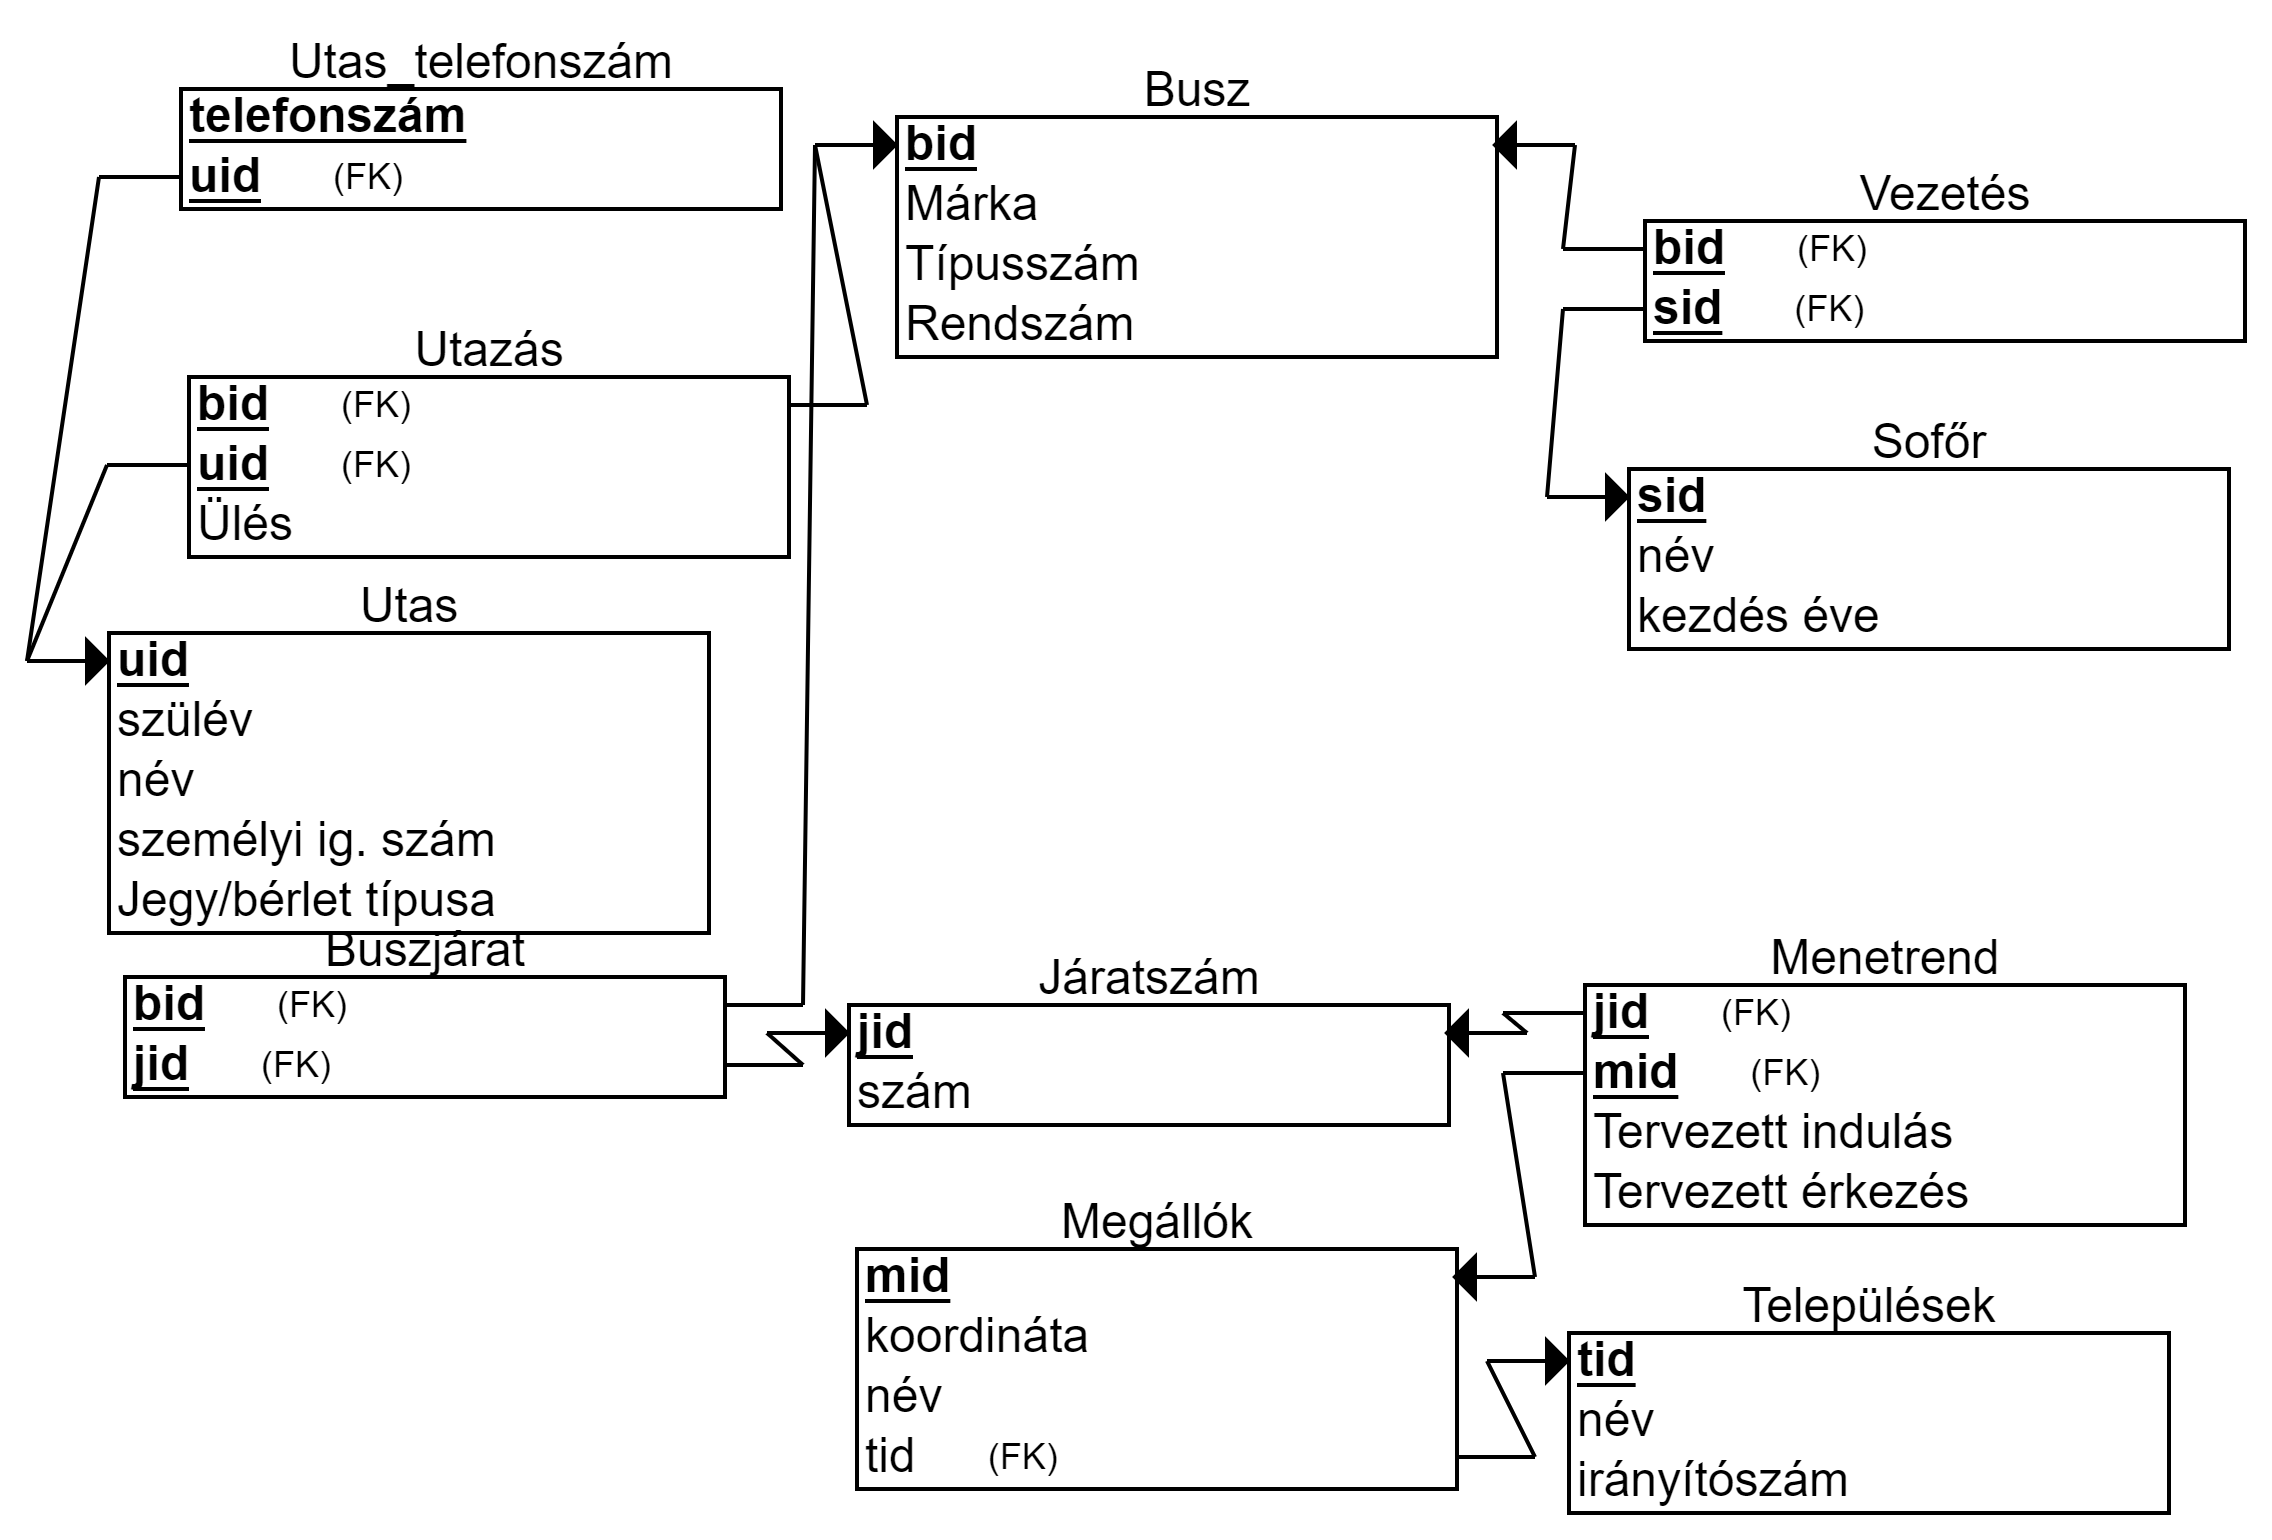
\includegraphics[height=10cm,width=15cm]{D:/Uni/Tex/Adatbázis beadandó/rs.png}
\newpage
\section{SQL}
\subsection{Adatbázis  létrehozása}
\begin{verbatim}
CREATE TABLE Utas(
    utid NUMBER(1) NOT NULL PRIMARY KEY,
    név varchar(30) NOT NULL,
    személyi_szám varchar(30) NOT NULL,
    jegy_bérlet_típis varchar(30) NOT NULL,
    szülév int NOT NULL
);
CREATE TABLE Utas_telefonszám(
    t_id NUMBER(1) NOT NULL PRIMARY KEY,
    telefonszám varchar(30),
    u_id NUMBER(1) NOT NULL,
    FOREIGN KEY (u_id) REFERENCES Utas(utid)
);
CREATE TABLE Járatszám(
    jid NUMBER(1) NOT NULL PRIMARY KEY,
    szám int NOT NULL
);
CREATE TABLE Utazás(
    ülés int,
    ut_id NUMBER(1) NOT NULL,
    FOREIGN KEY (ut_id) REFERENCES Utas(utid)
);
CREATE TABLE Sofőr(
    soid NUMBER(1) NOT NULL PRIMARY KEY,
    név varchar(30) NOT NULL,
    kezdés_éve int NOT NULL
);
CREATE TABLE Busz(
    bid NUMBER(1) NOT NULL PRIMARY KEY,
    márka varchar(30) NOT NULL,
    típusszám int NOT NULL,
    rendszám varchar(30) NOT NULL
);
CREATE TABLE Vezetés(
    s_id NUMBER(1) NOT NULL,
    b_id NUMBER(1) NOT NULL,
    FOREIGN KEY (s_id) REFERENCES Sofőr(soid),
    FOREIGN KEY (b_id) REFERENCES Busz(bid)
);
CREATE TABLE Települések(
    tid NUMBER(1) NOT NULL PRIMARY KEY,
    név varchar(30) NOT NULL,
    irányítószám int NOT NULL
);
CREATE TABLE Megállók(
    mid NUMBER(1) NOT NULL PRIMARY KEY,
    koordináta varchar(100) NOT NULL,
    név varchar(30) NOT NULL,
    t_id NUMBER(1) NOT NULL,
    FOREIGN KEY (t_id) REFERENCES Települések(tid)
);
CREATE TABLE Menetrend(
    tervezett_indulás_óra int,
    tervezett_indulás_perc int,
    tervezett_érkezés_óra int,
    tervezett_érkezés_perc int,
    j_id NUMBER(1) NOT NULL,
    m_id NUMBER(1) NOT NULL,
    FOREIGN KEY (j_id) REFERENCES Járatszám(jid),
    FOREIGN KEY (m_id) REFERENCES Megállók(mid)
);
CREATE TABLE Buszjárat(
    b_id NUMBER(1) NOT NULL,
    j_id NUMBER(1) NOT NULL,
    FOREIGN KEY (b_id) REFERENCES Busz(bid),
    FOREIGN KEY(j_id) REFERENCES Járatszám(jid)
);
\end{verbatim}
\newpage
\subsection{Adatbázis feltöltése}
\begin{verbatim}
INSERT INTO Utas VALUES(1,'Kiss Tamás','1356EA','Diák',2004);
INSERT INTO Utas_telefonszám VALUES(1,'06703459823',1);
INSERT INTO Járatszám VALUES(1,1359);
INSERT INTO Utazás VALUES(22,1);
INSERT INTO Sofőr VALUES(1,'Benedek Ferenc',2013);
INSERT INTO Busz VALUES(1,'Volvo',17346,'RGA-578');
INSERT INTO Vezetés VALUES(1,1);
INSERT INTO Települések VALUES(1,'Dunaharaszti',2330);
INSERT INTO Megállók VALUES(1,'12735E-2372737N','Dunaharaszti, Kisbolt',1);
INSERT INTO Menetrend VALUES(12,45,12,43,1,1);
INSERT INTO Buszjárat VALUES(1,1);
\end{verbatim}
\subsection{UPDATE parancsok}
Busz táblában a két rendszám megegyezik. Két busz van a táblában. A Volvo rendszáma hibás. Megoldás:
\begin{verbatim}
UPDATE Busz SET rendszám='DBA-972' WHERE rendszám like 'RGA-578' AND márka like 'Volvo'
\end{verbatim}
Járatszámnál 1-2 ID-vel rendelkezőknek ugyanaz a járatszáma, illetve 3-4-nek is. A 2-es ID-vel rendelkező legyen 980, a 4-es ID-vel rendelkező pedig legyen 1501.
\begin{verbatim}
UPDATE Járatszám SET szám=980 WHERE jid=2
UPDATE Járatszám SET szám=1501 WHERE jid=4
\end{verbatim}
Az Utas táblában el van írva a 
\begin{verbatim}jegy_bérlet_típus\end{verbatim}
Megoldás:
\begin{verbatim}
ALTER TABLE Utas RENAME COLUMN jegy_bérlet_típis TO jegy_bérlet_típus
\end{verbatim}
Utazás táblából hiányzik egy FK ami a Járatszámhoz kapcsolódik. Megoldás:
\begin{verbatim}
ALTER TABLE Utazás ADD ja_id int;
ALTER TABLE Utazás ADD FOREIGN KEY (ja_id) REFERENCES Járatszám(jid);
\end{verbatim}
Most hozzáadjuk a megfelelő értékeket:
\begin{verbatim}
UPDATE Utazás SET ja_id=1 WHERE ut_id=1;
UPDATE Utazás SET ja_id=2 WHERE ut_id=2;
UPDATE Utazás SET ja_id=3 WHERE ut_id=3;
\end{verbatim}
\newpage
\subsection{Select parancsok}
2000 előtt született Utasok:
\begin{spverbatim}
SELECT név from Utas WHERE szülév<2000;
\end{spverbatim}
2000 után született utasok száma:
\begin{spverbatim}
SELECT Count(név) from Utas WHERE szülév>2000
\end{spverbatim}
Taksony településnek az irányítószáma:
\begin{spverbatim}
SELECT irányítószám from Települések WHERE név like 'Taksony';
\end{spverbatim}
Az összes sofőr lekérdezése:
\begin{spverbatim}
SELECT név from Sofőr;
\end{spverbatim}
Összes sofőr lekérdezése aki 2010 előtt kezdett el dolgozni:
\begin{spverbatim}
SELECT név from Sofőr WHERE kezdés_éve<2010;
\end{spverbatim}
Teljes árú jegy/bérletet vett utasok neve:
\begin{spverbatim}
SELECT név from Utas WHERE jegy_bérlet_típus like 'Teljes árú';
\end{spverbatim}
Volvo típusú buszok rendszámának lekérdezése:
\begin{spverbatim}
SELECT rendszám from Busz WHERE márka like 'Volvo';
\end{spverbatim}
Az utasok között mennyi a diák?
\begin{spverbatim}
SELECT Count(*) from Utas WHERE jegy_bérlet_típus like 'Diák';
\end{spverbatim}
Az 1359-es járatszámú busznak hány megállója van?
\begin{spverbatim}
SELECT Count(*) from Járatszám JOIN Menetrend on jid=j_id JOIN Megállók ON m_id=mid WHERE szám=1359;
\end{spverbatim}
Az 1359-es járatszámú busznak megállóinak a nevei:
\begin{spverbatim}
SELECT Megállók.név from Járatszám JOIN Menetrend on jid=j_id JOIN Megállók ON m_id=mid WHERE szám=1359;
\end{spverbatim}
Dunaharasztin átmenő buszok járatszáma:
\begin{spverbatim}
SELECT szám from Járatszám JOIN Menetrend on jid=j_id JOIN Megállók ON m_id=mid JOIN Települések ON tid=t_id WHERE Települések.név like 'Dunaharaszti';
\end{spverbatim}
Hány busz megy át Taksony településen?
\begin{spverbatim}
SELECT Count(szám) from Járatszám JOIN Menetrend on jid=j_id JOIN Megállók ON m_id=mid JOIN Települések ON tid=t_id WHERE Települések.név like 'Taksony';
\end{spverbatim}
1359-es járatszámú buszon utazók száma:
\begin{spverbatim}
SELECT Count(*) from Járatszám JOIN Utazás ON jid=ja_id JOIN Utas on utid=ut_id WHERE szám=1359;
\end{spverbatim}
Ha tudjuk hogy egy járatszámú busz megy csak Taksonyba, akkor hány utas van rajta?
\begin{spverbatim}
SELECT Count(*) from Járatszám JOIN Utazás ON jid=ja_id JOIN Utas on utid=ut_id WHERE szám=(SELECT szám from Járatszám JOIN Menetrend on jid=j_id JOIN Megállók ON m_id=mid JOIN Települések ON tid=t_id WHERE Települések.név like 'Taksony');
\end{spverbatim}
\end{document}